%**************************************************************************
%*  Course project report, based on the ELCVIA LaTeX 2e template          *
%*  (Electronic Letters on Computer Vision and Image Analysis)            *
%*                                                                        *
%*  Build: pdflatex main -> bibtex main -> pdflatex main -> pdflatex main *
%*  The template style file elcvia.sty is in this folder.                 *
%*  Figures are read from ../results/ (see \graphicspath below).          *
%**************************************************************************

\documentclass[twoside,a4paper,11pt]{article}
\usepackage{times}
\usepackage{elcvia}
\usepackage[english]{babel}

% Packages used by the report sections (the template's psfig.sty is not needed: figures use graphicx)
\usepackage{graphicx}
\usepackage{booktabs}
\usepackage{amsmath}
\usepackage{amssymb}
\usepackage{url}
\usepackage{tikz}
\usetikzlibrary{arrows.meta}
\graphicspath{{../results/}{figures/}}

\newcommand{\Runo}{\rm I\hspace{-0.55ex}R}

% INFORMATION TO FILL IN CAMERA READY VERSION
%------------------------------------------------------------------
\newcommand{\vol}{0}            % Number of Volume (default 0)
\newcommand{\num}{0}            % Number (default 0)
\setcounter{page}{1}            % First page (default 1)
\newcommand{\begpag}{\thepage}
\newcommand{\finpag}{7}         % Last Page  TODO: set to the real last page
\newcommand{\yearp}{2026}       % Year of the issue
%------------------------------------------------------------------
\renewcommand{\thefootnote}{\fnsymbol{footnote}}

\title{Receipt Information Extraction with Layout-Aware Transformers:\\
How Much Does Layout Add over Text?
\footnote[0]{Correspondence to: hiranyapatil10@gmail.com, himanshuchundawat00@gmail.com \vspace{0.2cm}}
% INFORMATION TO FILL IN CAMERA READY VERSION
%------------------------------------------------------------------
% name of Associate Editor given when article is accepted
\footnote[0]{\noindent Recommended for acceptance by $<$name$>$}
%------------------------------------------------------------------
\footnote[0]{ELCVIA ISSN:1577-5097}
\footnote[0]{Published by Computer Vision Center / Universitat Aut\`onoma de
Barcelona, Barcelona, Spain}
}

\author{Hiranya Patil$^*$ and Himanshu Chundawat$^*$ \\ \\
\centerline{\small \em $^*$ Computer Science (B.Tech), Sitare University, Lucknow, India} \\ \\
% Submission date (replaces the template's received / revised / accepted dates)
\centerline{\small Submitted 22 November 2026}
       }


\begin{document}

\maketitle

\pagestyle{myheadings}

% INFORMATION TO FILL IN CAMERA READY VERSION
%-------------------------------------------------------------------
% fill in (authors) the authors of article in following format:
% * 1,2 authors: J. Jones and J. Jones
% * More than 2 authors: J. Jones et al.
\markboth{\centerline{\small \it H. Patil and H. Chundawat /
           Electronic Letters on Computer Vision and Image Analysis
           \vol(\num):\begpag-\finpag, \yearp}}
         {\centerline{\small \it H. Patil and H. Chundawat /
           Electronic Letters on Computer Vision and Image Analysis
           \vol(\num):\begpag-\finpag, \yearp}}
%-------------------------------------------------------------------
\hrulefill

\begin{abstract}

% abstract.tex
% TODO (chundawat-h): Abstract (3-5 sentences: task, dataset, three methods, main result: how much layout adds).

\textit{To be written.}


\vspace{0.5cm}
\noindent
{\em Key Words}: Document Analysis and OCR, Key Information Extraction,
Receipts, LayoutLM, BERT, Token Classification.

\end{abstract}
\hrulefill

% ---- chundawat-h ----
% introduction.tex (chundawat-h)

\section{Introduction}
\label{sec:intro}

Receipts and invoices are produced in huge numbers and are needed for
expense reports, bookkeeping and tax filing. Turning a scanned receipt
into structured data, such as \emph{who} sold, \emph{when} and for
\emph{how much}, is still often done by hand. Automating it is a classic
document-analysis task: an OCR engine first reads the words and their
positions, and a second step must decide which words belong to which
field.

The second step is harder than it looks. Receipts have no fixed
template: each shop places its name, address, date and total
differently, and the same receipt may print several candidate amounts
(item prices, subtotal, tax, total before and after rounding, cash
paid). OCR adds noise on top, for example splitting a number
(\texttt{39. 80}) or misreading characters (\texttt{SON BHD} for
\texttt{SDN BHD}).

Two kinds of information can help. The \emph{text} of a word and its
neighbours tells a model what the word is, while its \emph{layout}, the
position on the page, tells it where the word sits: company names are
usually at the top, and the total is usually on the same line as the
word ``TOTAL''. Pre-trained language models such as
BERT~\cite{devlin2019bert} use only the text. LayoutLM~\cite{xu2020layoutlm}
extends BERT with embeddings of each word's 2D bounding box and was
pre-trained on scanned documents.

\paragraph{Problem statement.} Given the OCR words and bounding boxes of
a scanned receipt, extract one string for each of four fields:
\emph{company}, \emph{date}, \emph{address} and \emph{total}.

\paragraph{Research question.} How much does layout information add
over text alone, and for which fields? We answer this with a field-wise
$F_1$ comparison of three methods that use the same OCR input:
\begin{enumerate}
  \item a rule-based \textbf{regex baseline} (text and line order, no learning);
  \item \textbf{BERT} token classification (text only);
  \item \textbf{LayoutLM} token classification (text and 2D position).
\end{enumerate}
BERT and LayoutLM have the same size, vocabulary and training settings,
so the difference between them isolates the effect of the layout input.

\paragraph{Contributions.}
\begin{itemize}
  \item A reproducible comparison of rules, a text-only Transformer and a
        layout-aware Transformer on SROIE, with all code, predictions and
        notebooks publicly available.
  \item A field-wise analysis of where layout helps, with a paired
        bootstrap significance test and error examples: layout fixes
        block-boundary errors on company and address but does not help
        the total.
  \item A two-gold evaluation that separates model errors from OCR
        errors: even perfect word tagging scores only 82.8\% macro $F_1$
        against the official answers.
\end{itemize}

% related_work.tex (chundawat-h)

\section{Related work}
\label{sec:related}

\paragraph{Receipt and form understanding.} The ICDAR 2019 Robust
Reading Challenge on Scanned Receipts OCR and Information Extraction
(SROIE)~\cite{huang2019sroie} introduced a public benchmark of about
1{,}000 scanned receipts with three tasks: text localisation, OCR, and
key information extraction of company, date, address and total.
CORD~\cite{park2019cord} provides a larger receipt dataset with more
fine-grained labels. Before Transformers, such fields were usually
extracted with hand-crafted rules and templates, which work well for
fixed layouts but break on unseen ones.

\paragraph{Sequence labelling.} Key information extraction is commonly
framed as named-entity-style token classification with BIO
tags~\cite{ramshaw1995text}: each word is labelled as the Beginning or
Inside of a field, or Outside any field. Neural taggers such as the
BiLSTM-CRF~\cite{lample2016ner} became the standard approach and were
later replaced by fine-tuned Transformers~\cite{vaswani2017attention}.

\paragraph{Pre-trained language models.} BERT~\cite{devlin2019bert} is a
Transformer encoder pre-trained on large text corpora with masked
language modelling. Adding a classification layer and fine-tuning on
labelled tokens gives strong results on entity recognition. However,
BERT reads a document as a 1D sequence and cannot see where a word is on
the page.

\paragraph{Layout-aware models.} Chargrid~\cite{katti2018chargrid}
encodes a document as a 2D grid of characters for a convolutional
network. LayoutLM~\cite{xu2020layoutlm} keeps the BERT architecture and
adds 2D position embeddings of each word's bounding box. It was
pre-trained on 11 million scanned document pages and reported large
gains over BERT on form understanding and on SROIE.
LayoutLMv2~\cite{xu2021layoutlmv2} further adds visual features from the
page image. We use LayoutLM (v1) because it differs from BERT
\emph{only} in the layout input, which makes the comparison clean.


% ---- Hiranya ----
% Dataset section (Hiranya, issue #8)
% Needs: graphicx, booktabs, url (or hyperref). Figures are read from results/ (see \graphicspath in main.tex).

\section{Dataset}
\label{sec:dataset}

We use SROIE, the Scanned Receipts OCR and Information Extraction dataset of the ICDAR 2019 Robust Reading Challenge~\cite{huang2019sroie}. It contains scanned English-language receipts from Malaysia, and the key information extraction task (Task~3) asks for four fields per receipt: \emph{company}, \emph{date}, \emph{address} and \emph{total}. We use the standard split of 626 training and 347 test receipts.

\paragraph{Two versions of the same receipts.}
We combine two Hugging Face releases of SROIE, which contain the same receipt scans:
\begin{itemize}
  \item \texttt{darentang/sroie}\footnote{\url{https://huggingface.co/datasets/darentang/sroie}} provides, for every receipt, the OCR words, one bounding box per word already scaled to a $0$--$1000$ grid, and one BIO tag per word~\cite{ramshaw1995text}. With the label \texttt{O} and a \texttt{B-}/\texttt{I-} tag for each of the four fields, there are 9 labels. We use these tags to train BERT and LayoutLM and to build the main gold standard.
  \item \texttt{jsdnrs/ICDAR2019-SROIE}\footnote{\url{https://huggingface.co/datasets/jsdnrs/ICDAR2019-SROIE}} provides the receipt images and the official ICDAR answer strings for the four fields. It has no per-word tags. We use it for figures and for a second evaluation against the official answers.
\end{itemize}
The two are joined on the receipt key, the image file name (e.g.\ \texttt{X00016469612}). Every receipt in \texttt{darentang/sroie} has a match. The official test split contains 14 additional receipts that have no word tags; we leave them out so that all methods are evaluated on the same 347 test receipts. Figure~\ref{fig:receipt} shows a receipt with its word boxes coloured by label.

\begin{figure}[t]
  \centering
  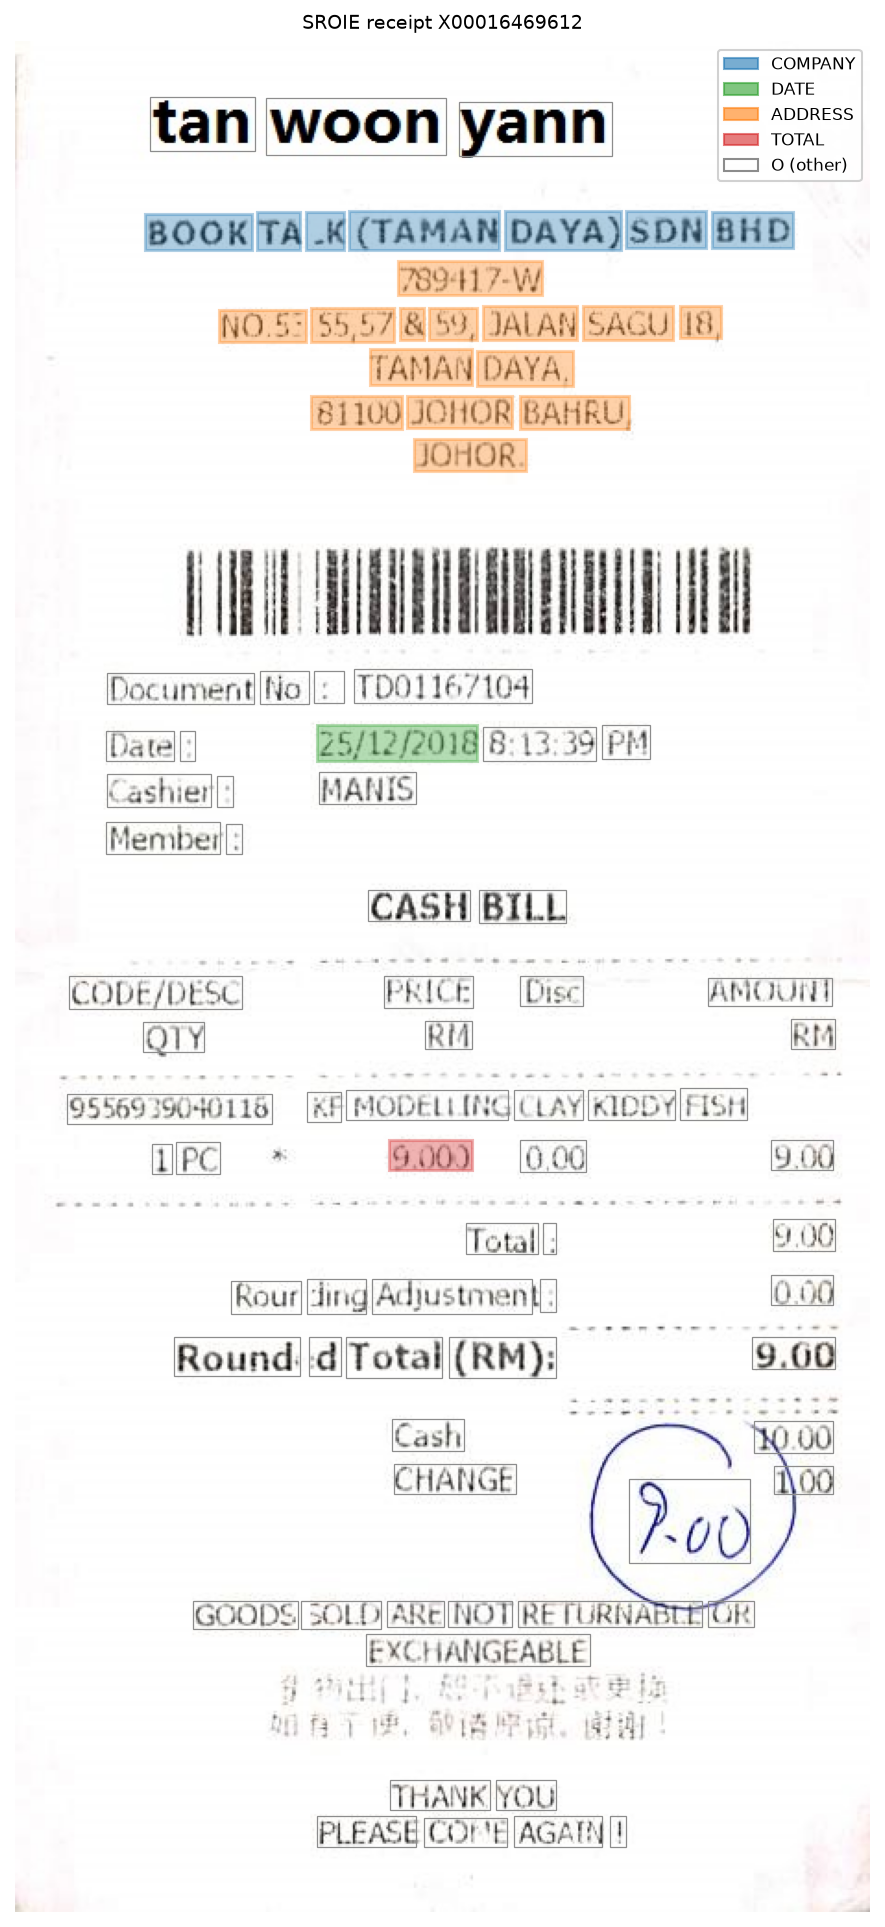
\includegraphics[width=0.36\linewidth]{receipt_example_1.png}
  \caption{A training receipt (\texttt{X00016469612}) with each OCR word box coloured by its tag: company (blue), address (orange), date (green), total (red), other (grey outline). The boxes are stored on a $0$--$1000$ grid and scaled back to pixels here; they line up with the printed words. The TOTAL tag sits on the item price \texttt{9.000} instead of the \texttt{9.00} on the total line (see Limitations).}
  \label{fig:receipt}
\end{figure}

\paragraph{Statistics.}
A receipt has $117.8$ OCR words on average in the training split ($116.5$ in the test split), ranging from 31 to 246. Most words are not part of any field: the label \texttt{O} covers $84.7\%$ of all words (Table~\ref{tab:labels} and Figure~\ref{fig:labels}). Every field is tagged exactly once per receipt as a single contiguous span, and all four fields are present in every receipt except one training receipt without an address. Address spans are the longest ($11.3$ words on average), company spans have $4.3$ words, and date and total are usually a single word.

\begin{table}[t]
  \centering
  \small
  \begin{tabular}{lrrr}
    \toprule
    Label & Train & Test & Share (\%) \\
    \midrule
    \texttt{O}         & 62{,}469 & 34{,}216 & 84.7 \\
    \texttt{B-COMPANY} &      626 &      347 &  0.9 \\
    \texttt{I-COMPANY} &  2{,}095 &  1{,}144 &  2.8 \\
    \texttt{B-DATE}    &      626 &      347 &  0.9 \\
    \texttt{I-DATE}    &      112 &       81 &  0.2 \\
    \texttt{B-ADDRESS} &      625 &      347 &  0.9 \\
    \texttt{I-ADDRESS} &  6{,}519 &  3{,}560 &  8.8 \\
    \texttt{B-TOTAL}   &      626 &      347 &  0.9 \\
    \texttt{I-TOTAL}   &       49 &       22 &  0.1 \\
    \midrule
    Receipts           &      626 &      347 &      \\
    Words              & 73{,}747 & 40{,}411 &      \\
    \bottomrule
  \end{tabular}
  \caption{Word-level label counts. The share is computed over both splits together.}
  \label{tab:labels}
\end{table}

\begin{figure}[t]
  \centering
  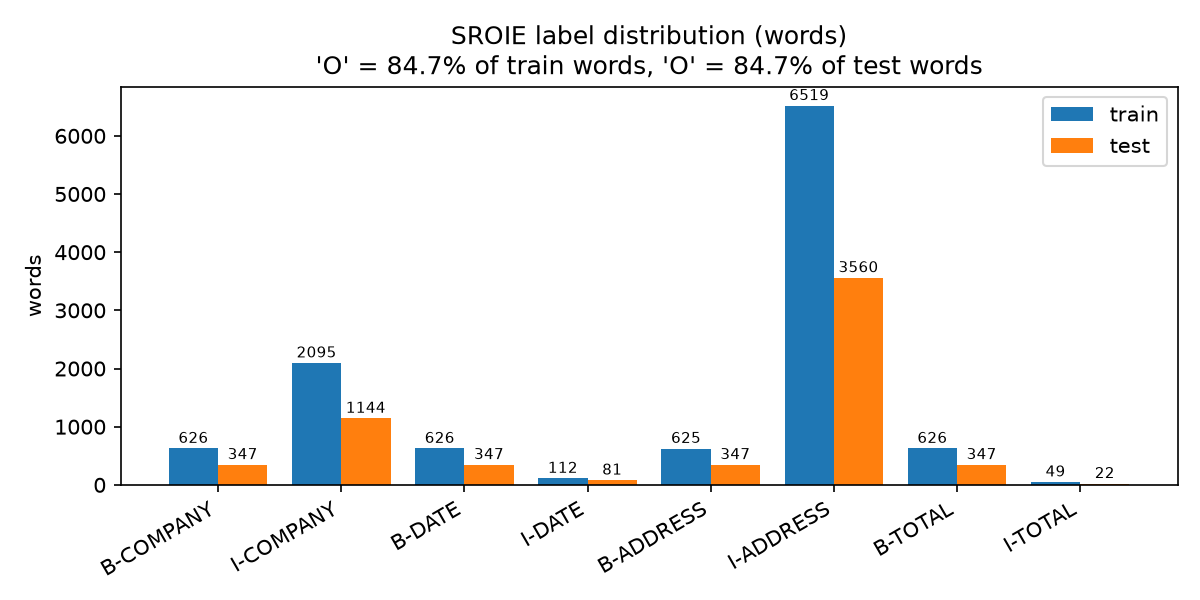
\includegraphics[width=0.7\linewidth]{label_distribution.png}
  \caption{Distribution of the field labels (words). \texttt{O}, not shown, makes up $84.7\%$ of all words.}
  \label{fig:labels}
\end{figure}

\paragraph{Sequence length.}
BERT and LayoutLM split words into WordPiece sub-tokens and read at most 512 of them. A receipt has about 257 sub-tokens on average ($2.2$ per word). Only 4 training receipts and 1 test receipt are longer than 512, and the words lost to truncation are never field words.

\paragraph{Limitations of the labels.}
The word tags were produced by matching the official answers against the OCR text, which leaves some noise:
\begin{itemize}
  \item \textbf{Total.} The total amount is usually printed several times (item price, subtotal, total line, cash), and $70\%$ of training receipts repeat its exact string. The tag is placed on the \emph{first} matching word in $96\%$ of the receipts, and only $67\%$ of TOTAL tags lie on a line that contains a word such as ``total'' or ``amount''. The layout cue ``the total is on the line that says TOTAL'' is therefore weaker in the labels than on the receipts.
  \item \textbf{Address and date.} Some address spans also include the company registration number (e.g.\ \texttt{789417-W} in Figure~\ref{fig:receipt}), and $2.6\%$ of date spans include extra words such as \texttt{Date:} or a time.
  \item \textbf{OCR noise.} The tagged words are OCR output, while the official answers were typed by annotators. Even a perfect tagger, scored against the official answers, would therefore not reach $100\%$ (Table~\ref{tab:ceiling}). The gap is largest for the address, where OCR spacing and misread characters (e.g.\ \texttt{SON BHD} for \texttt{SDN BHD}) break the exact match. For this reason our main evaluation uses the gold strings built from the word tags, and we report the official answers as a second score.
\end{itemize}

\begin{table}[t]
  \centering
  \small
  \begin{tabular}{lcc}
    \toprule
    Field & Exact match (\%) & Exact, ignoring spaces (\%) \\
    \midrule
    Company   & 80.4 & 80.7 \\
    Date      & 96.3 & 96.3 \\
    Address   & 58.2 & 74.4 \\
    Total     & 96.3 & 96.3 \\
    \midrule
    Macro avg & 82.8 & 86.9 \\
    \bottomrule
  \end{tabular}
  \caption{Upper bound for any tagging model scored against the official answers: the strings built from the gold word tags, compared with the official answers after the same normalisation as our evaluation (test split).}
  \label{tab:ceiling}
\end{table}


\section{Methods}
\label{sec:methods}
% ---- chundawat-h ----
% method_regex.tex
% TODO (chundawat-h): Method 1: rule-based baseline (src/regex_baseline.py, notebook 02).

\subsection{Method 1: OCR + regex baseline}
\label{sec:regex}

\textit{To be written.}

% ---- Hiranya ----
% Method 2: BERT (Hiranya, issue #8)
% Needs: amsmath, amssymb.

\subsection{Method 2: BERT token classification (text only)}
\label{sec:bert}

We cast extraction as sequence labelling: every OCR word of a receipt receives one of the 9 BIO labels (Section~\ref{sec:dataset}), and the words of each field are then joined into a string. As the text-only model we fine-tune \texttt{bert-base-uncased}~\cite{devlin2019bert} (12 layers, hidden size 768, about 110M parameters).

\paragraph{Input.}
The OCR words of a receipt are concatenated in the dataset's reading order and tokenised into WordPiece sub-tokens~\cite{wu2016google}, e.g.\ \texttt{25/12/2018} $\rightarrow$ \texttt{25}, \texttt{/}, \texttt{12}, \texttt{/}, \texttt{2018}. The sequence is framed by \texttt{[CLS]} and \texttt{[SEP]} and truncated to 512 sub-tokens. The model sees only the text; the position of a sub-token is just its index in this sequence.

\paragraph{Label alignment.}
Labels are defined per word, but the model predicts per sub-token. As is standard for BERT~\cite{devlin2019bert}, only the \emph{first} sub-token of each word carries the word's label. All other sub-tokens and the special tokens receive the ignore index, so they do not contribute to the loss.

\paragraph{Model and loss.}
A linear layer on top of the final hidden state $\mathbf{h}_t \in \mathbb{R}^{768}$ of each sub-token $t$ produces a distribution over the $K=9$ labels,
\begin{equation}
  p(y_t \mid \text{receipt}) = \operatorname{softmax}\!\left(\mathbf{W}\mathbf{h}_t + \mathbf{b}\right), \qquad \mathbf{W} \in \mathbb{R}^{K \times 768},
\end{equation}
and the whole network is fine-tuned with the cross-entropy loss averaged over the labelled sub-tokens $\mathcal{T}$ (the first sub-token of each word):
\begin{equation}
  \mathcal{L} = -\frac{1}{|\mathcal{T}|} \sum_{t \in \mathcal{T}} \log p(y_t^{*} \mid \text{receipt}).
\end{equation}

\paragraph{From predictions to fields.}
At test time each word takes the label predicted for its first sub-token, and words removed by truncation are labelled \texttt{O}. This gives one label per word, in the same format as the gold tags. The words of each field are grouped into spans (a \texttt{B-} tag, or an \texttt{I-} tag that does not continue the current field, starts a new span), and the spans are joined with spaces into one string per field. The same conversion is applied to the gold tags, so the predictions and the main gold standard are built in exactly the same way.

% Method 3: LayoutLM (Hiranya, issue #8)
% Needs: amsmath, amssymb, tikz with \usetikzlibrary{arrows.meta}, graphicx (for \resizebox).

\subsection{Method 3: LayoutLM (text + 2D layout)}
\label{sec:layoutlm}

LayoutLM~\cite{xu2020layoutlm} extends BERT with the position of each token on the page. A receipt is not free text: the company name is at the top, the date follows a ``Date:'' label on the same line, and the total sits at the right end of the line that says ``TOTAL''. LayoutLM can use these cues, while BERT only knows the order of the words. We fine-tune \texttt{microsoft/layoutlm-base-uncased}, which has the same architecture and size as BERT-base (12 layers, hidden size 768) and the same uncased WordPiece vocabulary. It was initialised from BERT-base and then pre-trained on about 11 million scanned document pages from the IIT-CDIP collection, where it learned to predict masked words from their text and layout context~\cite{xu2020layoutlm}.

\paragraph{Text and 2D position embeddings.}
Each word $w$ comes with a bounding box $(x_0, y_0, x_1, y_1)$ on a $0$--$1000$ grid, where $(x_0, y_0)$ is the top-left and $(x_1, y_1)$ the bottom-right corner. Every sub-token inherits the box of its word. LayoutLM adds 2D position embeddings to BERT's input embedding of sub-token $t$:
\begin{equation}
\begin{aligned}
  \mathbf{e}_t ={}& \mathbf{E}_{\text{tok}}[w_t] + \mathbf{E}_{\text{pos}}[t] + \mathbf{E}_{\text{seg}}[0] \\
  &+ \mathbf{E}_{x}[x_0] + \mathbf{E}_{y}[y_0] + \mathbf{E}_{x}[x_1] + \mathbf{E}_{y}[y_1] \\
  &+ \mathbf{E}_{h}[y_1 - y_0] + \mathbf{E}_{w}[x_1 - x_0].
\end{aligned}
\end{equation}
The first line is BERT's input embedding (token, 1D position and segment). The other two lines are the 2D position embeddings added by LayoutLM: $\mathbf{E}_{x}$ and $\mathbf{E}_{y}$ are learned tables for horizontal and vertical coordinates (shared between the two corners), and $\mathbf{E}_{h}$, $\mathbf{E}_{w}$ embed the box height and width. The sum is normalised and passed through the same Transformer encoder as in BERT, so self-attention can relate words by both their meaning and their position on the receipt. The special tokens get fixed boxes: \texttt{[CLS]} $\rightarrow (0,0,0,0)$, \texttt{[SEP]} $\rightarrow (1000,1000,1000,1000)$, and padding $\rightarrow (0,0,0,0)$. Figure~\ref{fig:layoutlm} shows the input for three words of the example receipt.

The original paper also proposes adding image features from a Faster R-CNN for some tasks~\cite{xu2020layoutlm}. We do not use them: our LayoutLM receives exactly the same words and labels as BERT plus the boxes, so the difference between the two models measures the contribution of layout alone.

\paragraph{Training and prediction.}
Everything else is identical to BERT (Section~\ref{sec:bert}): the same 9-label linear classifier on each final hidden state, the same first-sub-token label alignment and cross-entropy loss, the same truncation to 512 sub-tokens, and the same conversion from word labels to field strings. The boxes are padded together with the text, using $(0,0,0,0)$ for padding positions.

\begin{figure}[t]
  \centering
  \resizebox{\linewidth}{!}{%
  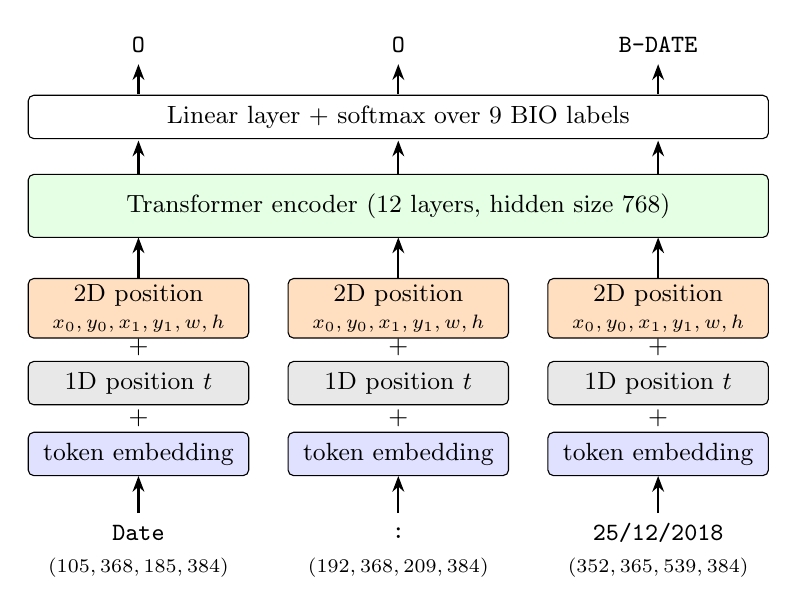
\begin{tikzpicture}[
      font=\small,
      emb/.style={draw, rounded corners=2pt, minimum width=2.8cm, minimum height=0.55cm, align=center, inner sep=2pt},
      textemb/.style={emb, fill=blue!12},
      posemb/.style={emb, fill=gray!18},
      boxemb/.style={emb, fill=orange!25, minimum height=0.75cm},
      wide/.style={draw, rounded corners=2pt, minimum width=9.4cm, align=center},
      arr/.style={-{Stealth[length=2mm]}, thick},
    ]
    % ---- input words and their boxes (receipt X00016469612) ----
    \node at (0,0)   {\texttt{Date}};
    \node at (3.3,0) {\texttt{:}};
    \node at (6.6,0) {\texttt{25/12/2018}};
    \node[font=\scriptsize] at (0,-0.45)   {$(105, 368, 185, 384)$};
    \node[font=\scriptsize] at (3.3,-0.45) {$(192, 368, 209, 384)$};
    \node[font=\scriptsize] at (6.6,-0.45) {$(352, 365, 539, 384)$};
    % ---- embeddings, summed per token ----
    \foreach \x in {0, 3.3, 6.6} {
      \draw[arr] (\x,0.25) -- (\x,0.72);
      \node[textemb] at (\x,1.0)  {token embedding};
      \node at (\x,1.45) {$+$};
      \node[posemb]  at (\x,1.9)  {1D position $t$};
      \node at (\x,2.35) {$+$};
      \node[boxemb]  at (\x,2.85) {2D position\\[-1pt]{\scriptsize $x_0, y_0, x_1, y_1, w, h$}};
      \draw[arr] (\x,3.23) -- (\x,3.75);
      \draw[arr] (\x,4.55) -- (\x,4.98);
      \draw[arr] (\x,5.57) -- (\x,5.95);
    }
    % ---- shared encoder and classifier ----
    \node[wide, minimum height=0.8cm, fill=green!10] at (3.3,4.15) {Transformer encoder (12 layers, hidden size 768)};
    \node[wide, minimum height=0.55cm] at (3.3,5.28) {Linear layer + softmax over 9 BIO labels};
    % ---- outputs ----
    \node at (0,6.2)   {\texttt{O}};
    \node at (3.3,6.2) {\texttt{O}};
    \node at (6.6,6.2) {\texttt{B-DATE}};
  \end{tikzpicture}%
  }
  \caption{LayoutLM input for three words of the receipt in Figure~\ref{fig:receipt}, with their boxes on the $0$--$1000$ grid. Each token's input is the sum of its token, 1D position and 2D position embeddings. BERT is the same model without the orange 2D position embedding. For simplicity one token per word is shown; in practice \texttt{25/12/2018} is split into five sub-tokens that all share the word's box, and only the first one is labelled.}
  \label{fig:layoutlm}
\end{figure}

% Experimental setup (Hiranya, issue #8)
% Needs: booktabs, graphicx. Numbers from results/bert_hparams.json, results/layoutlm_hparams.json and the training logs.

\section{Experimental setup}
\label{sec:setup}

\paragraph{Implementation and hardware.}
Both models are fine-tuned with the Hugging Face Transformers library~\cite{wolf2020transformers} (version 5.22.1) and PyTorch 2.14.1, using its \texttt{Trainer}. We trained on Google Colab on a single NVIDIA Tesla T4 GPU with mixed-precision (fp16) training. The code is in the notebooks \texttt{03\_bert\_text\_only.ipynb} and \texttt{04\_layoutlm.ipynb}, with shared data loading and evaluation code in \texttt{src/}.

\paragraph{Hyperparameters.}
BERT and LayoutLM use exactly the same hyperparameters (Table~\ref{tab:hparams}). They were fixed in advance and not tuned. The LayoutLM notebook reads them from the saved BERT configuration and stops if any value differs, so the two runs cannot drift apart. Both models are base-size Transformers of the same depth and width, start from pre-trained weights, and add a randomly initialised 9-label classifier.

\begin{table}[t]
  \centering
  \small
  \begin{tabular}{ll}
    \toprule
    Hyperparameter & Value (both models) \\
    \midrule
    Pre-trained model   & \texttt{bert-base-uncased} / \texttt{microsoft/layoutlm-base-uncased} \\
    Max.\ sequence length & 512 sub-tokens \\
    Optimiser           & AdamW~\cite{loshchilov2019adamw} \\
    Learning rate       & $5 \times 10^{-5}$, linear decay, no warm-up \\
    Weight decay        & 0 \\
    Batch size          & 8 receipts \\
    Epochs              & 10 (790 optimisation steps) \\
    Precision           & fp16 mixed precision \\
    Random seed         & 42 \\
    \midrule
    Training time (T4)  & BERT 2.3 min, LayoutLM 2.5 min \\
    \bottomrule
  \end{tabular}
  \caption{Training configuration, shared by both models.}
  \label{tab:hparams}
\end{table}

\paragraph{Training protocol.}
SROIE has no official validation split, and with only 626 training receipts we did not set one aside. Instead, both models are trained on the full training split for the fixed number of epochs. There is no early stopping and no checkpoint selection, and the test split is used exactly once, after training. No model weights are kept. Figure~\ref{fig:loss} shows that both models fit the training data smoothly: the training loss falls from about 1 to about 0.003 by the end of training, and LayoutLM's loss is slightly lower than BERT's for most of the run.

\begin{figure}[t]
  \centering
  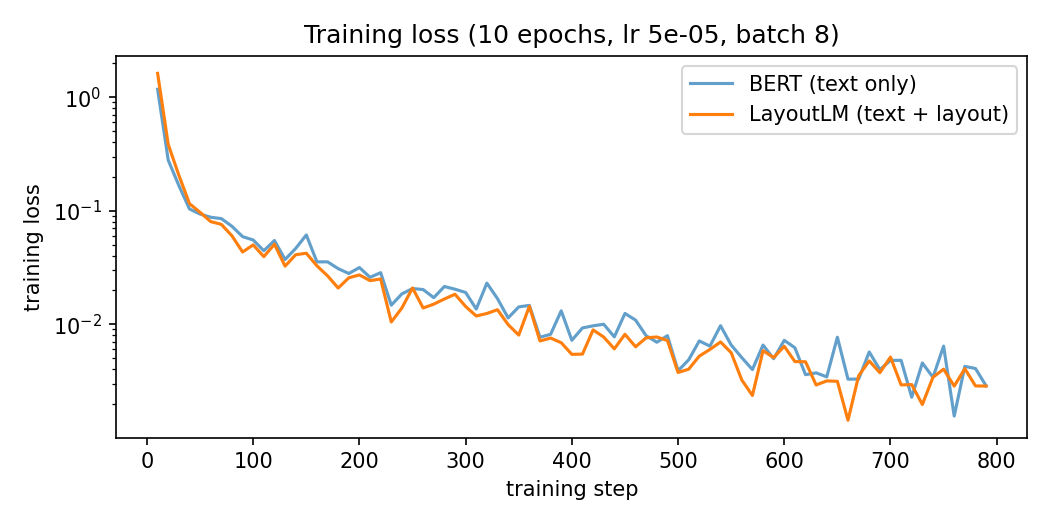
\includegraphics[width=0.7\linewidth]{layoutlm_training_loss.png}
  \caption{Training loss (log scale) of BERT and LayoutLM, logged every 10 steps, with identical hyperparameters.}
  \label{fig:loss}
\end{figure}

\paragraph{Evaluation.}
All three methods (regex, BERT, LayoutLM) are scored with the same field-level evaluation on the 347 test receipts. For each receipt and field, the predicted string is compared with the gold string after normalisation: lowercase, collapse whitespace, strip punctuation at both ends, and for the total also remove a currency prefix (\texttt{RM}) and thousands separators. A prediction is correct only if the two strings are then identical. Per field we report
\begin{equation}
  P = \frac{\#\text{correct}}{\#\text{non-empty predictions}}, \quad
  R = \frac{\#\text{correct}}{\#\text{non-empty gold}}, \quad
  F_1 = \frac{2PR}{P + R},
\end{equation}
and the macro average over the four fields. We use two gold standards (Section~\ref{sec:dataset}). The \emph{main} gold is the string built from the gold word tags, which measures whether a method picks the right words. The \emph{second} gold is the official ICDAR answers; there, even a perfect tagger is capped by OCR noise (Table~\ref{tab:ceiling}). For the two neural models we also report entity-level precision, recall and $F_1$ on the word tags with \texttt{seqeval}~\cite{nakayama2018seqeval}.

\paragraph{Limitations of the setup.}
Each model was trained once with a single seed. Differences of about one $F_1$ point between BERT and LayoutLM on a single field may therefore be within run-to-run variation; repeating the runs with several seeds would make the comparison more robust.


% ---- chundawat-h ----
% results.tex (chundawat-h)
% Numbers from notebooks/05_results_analysis.ipynb and results/final_results*.csv,
% layout_gain_bootstrap.csv, bert_vs_layoutlm_wins.csv, error_types.csv.

\section{Results and analysis}
\label{sec:results}

\subsection{Main results}

Table~\ref{tab:main} compares the three methods against the main gold
and Table~\ref{tab:official} against the official answers;
Figure~\ref{fig:f1} shows both.

\begin{table}[t]
  \centering
  \small
  \begin{tabular}{lccccc}
    \toprule
    Field     & Regex & BERT & LayoutLM & Layout gain & 95\% CI of gain \\
    \midrule
    Company   & 68.3 & 89.3 & \textbf{92.9} & $+3.6$ & $[0.9, 6.5]$ \\
    Date      & 95.8 & 97.8 & \textbf{98.7} & $+0.9$ & $[0.0, 2.0]$ \\
    Address   & 59.9 & 91.1 & \textbf{93.7} & $+2.6$ & $[0.9, 4.6]$ \\
    Total     & 75.2 & 89.4 & \textbf{89.5} & $+0.1$ & $[-3.1, 3.6]$ \\
    \midrule
    Macro avg & 74.8 & 91.9 & \textbf{93.7} & $+1.8$ & $[0.5, 3.2]$ \\
    \bottomrule
  \end{tabular}
  \caption{Test $F_1$ (\%) against the main gold (347 receipts). Layout
  gain = LayoutLM $-$ BERT, with its 95\% confidence interval from a
  paired bootstrap over receipts (2{,}000 resamples).}
  \label{tab:main}
\end{table}

\begin{table}[t]
  \centering
  \small
  \begin{tabular}{lcccc}
    \toprule
    Field     & Regex & BERT & LayoutLM & Ceiling \\
    \midrule
    Company   & 57.6 & 72.8 & \textbf{75.2} & 80.4 \\
    Date      & 95.8 & 95.0 & \textbf{96.1} & 96.3 \\
    Address   & 40.9 & 55.6 & \textbf{57.1} & 58.2 \\
    Total     & 77.2 & \textbf{86.5} & 86.0 & 96.3 \\
    \midrule
    Macro avg & 67.9 & 77.5 & \textbf{78.6} & 82.8 \\
    \bottomrule
  \end{tabular}
  \caption{Test $F_1$ (\%) against the official ICDAR answers. Ceiling =
  perfect word tagging (Table~\ref{tab:ceiling}).}
  \label{tab:official}
\end{table}

\begin{figure}[t]
  \centering
  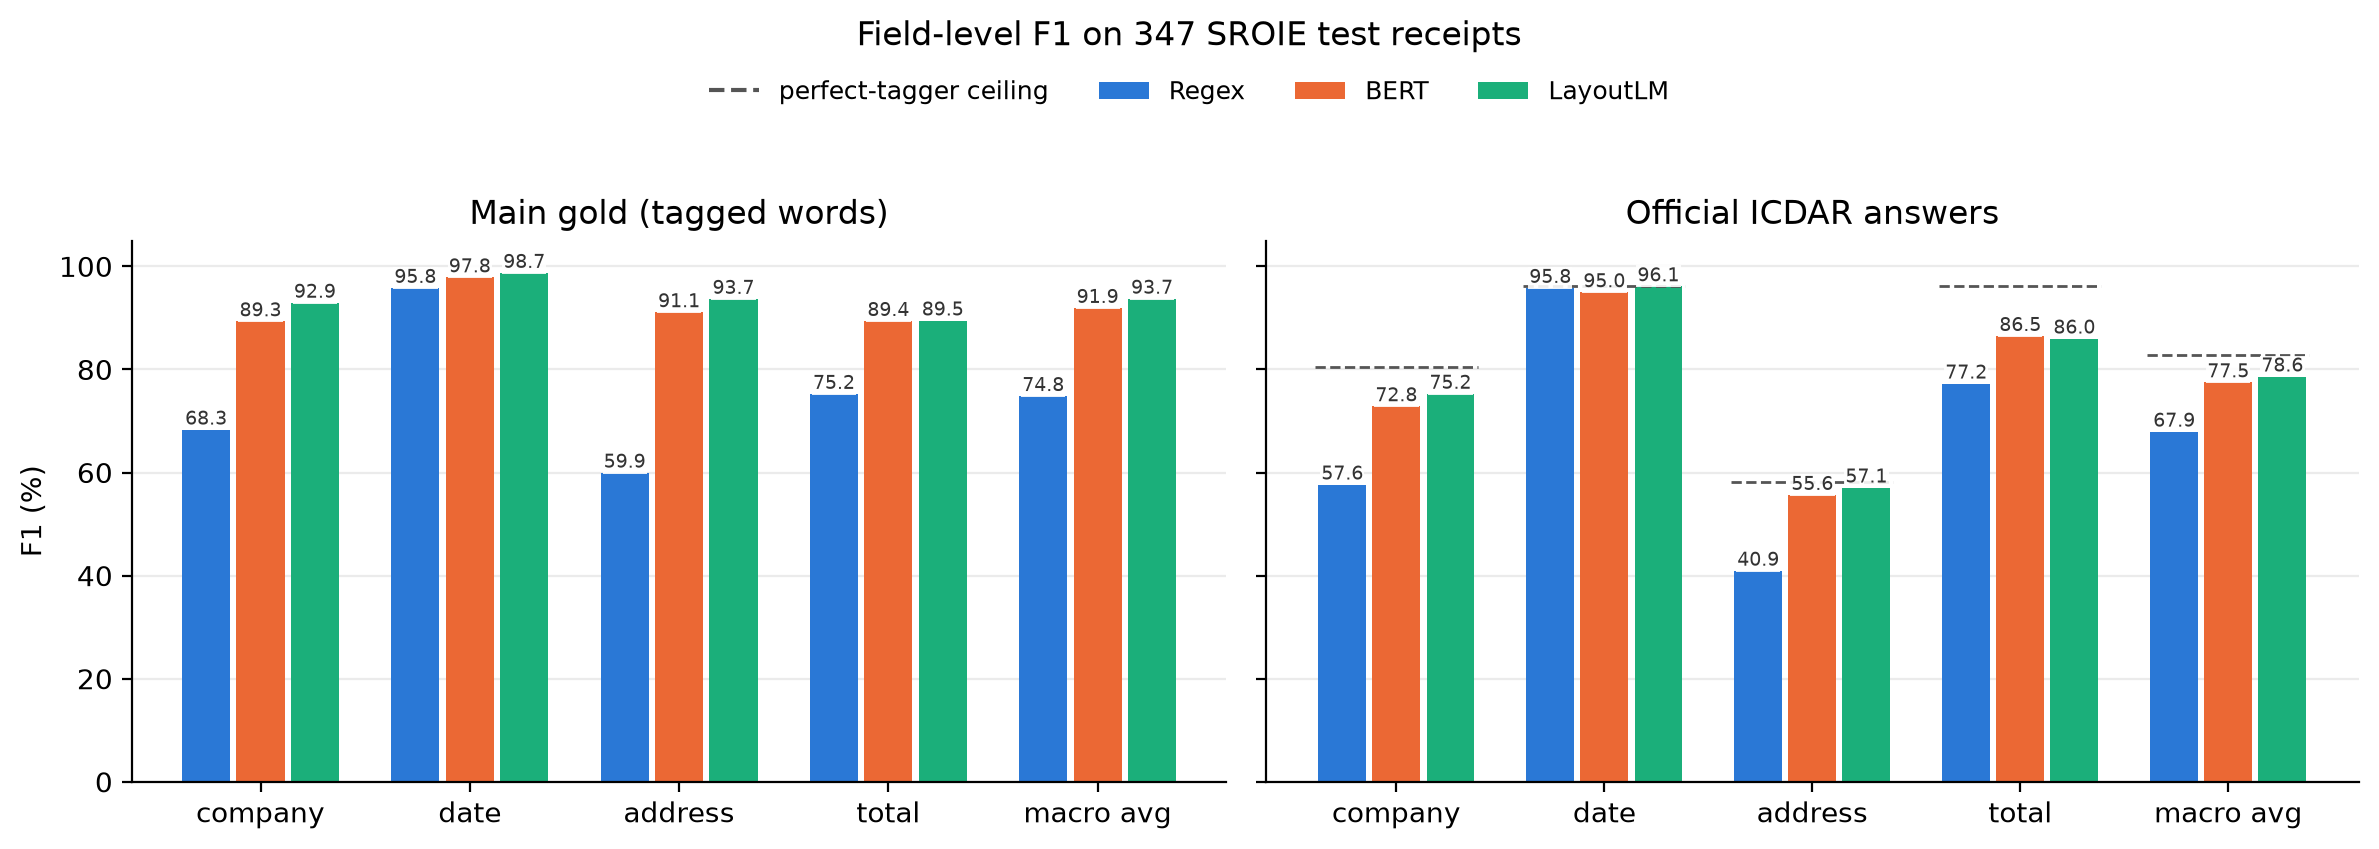
\includegraphics[width=\linewidth]{f1_comparison.png}
  \caption{Per-field test $F_1$ of the three methods against the main
  gold (left) and the official answers (right). Dashed lines mark the
  perfect-tagging ceiling.}
  \label{fig:f1}
\end{figure}

\subsection{Regex baseline}

The baseline reaches 74.8\% macro $F_1$ (76.7\% on the training split it
was tuned on, so it is not over-fitted). Its strengths and failures are
clear-cut:
\begin{itemize}
  \item \textbf{Date} (95.8\%) is almost solved by patterns, because
        dates have a fixed, distinctive format. Most remaining errors are
        label artefacts: some gold date spans include extra words such
        as \texttt{Date:} or a time (Section~\ref{sec:dataset}), which
        the regex correctly leaves out.
  \item \textbf{Total} (75.2\%) fails when a receipt prints several
        totals (before and after rounding, inside GST summary tables) or
        when OCR splits a number.
  \item \textbf{Company} (68.3\%) fails when other text sits above the
        name (\texttt{*** COPY ***}, the cashier's name) or when the name
        has no keyword such as \texttt{SDN BHD}.
  \item \textbf{Address} (59.9\%) is the hardest: its start and end vary,
        and the labels are not consistent about including registration
        numbers or trailing lines.
\end{itemize}

\subsection{Text only vs.\ text + layout}

\paragraph{Learning vs.\ rules.} Text-only BERT improves macro $F_1$ by
17.1 points over the rules ($74.8 \rightarrow 91.9$). The largest gains
are on the free-form fields, address ($+31.1$) and company ($+21.0$),
where rules cannot know where a block starts and ends. Date gains only
2 points because patterns already solve it.

\paragraph{Layout gain.} With the same tokenizer, data and
hyperparameters, adding 2D positions raises macro $F_1$ by a further 1.8
points, to 93.7\%. Because the test set is small, we estimate the
uncertainty with a paired bootstrap: we resample the 347 receipts with
replacement 2{,}000 times and recompute both models' $F_1$ on each
resample. The macro gain is positive in 99.6\% of resamples (95\% CI
$[0.5, 3.2]$). Per field (Table~\ref{tab:main}), the gain is clearly
positive for company ($+3.6$) and address ($+2.6$), borderline for date
($+0.9$) and zero for total ($+0.1$, CI $[-3.1, 3.6]$).
Table~\ref{tab:wins} shows the same picture per receipt: on company and
address, LayoutLM fixes many more receipts than it breaks, while on the
total the two models simply make \emph{different} mistakes (22 vs.\ 23
receipts).

\begin{table}[t]
  \centering
  \small
  \begin{tabular}{lcccc}
    \toprule
     & Company & Date & Address & Total \\
    \midrule
    Only LayoutLM correct & 20 & 4 & 10 & 22 \\
    Only BERT correct     &  8 & 1 &  1 & 23 \\
    Both correct          & 301 & 338 & 315 & 284 \\
    Both wrong            & 18 & 4 & 21 & 18 \\
    \bottomrule
  \end{tabular}
  \caption{Receipt-level agreement of BERT and LayoutLM on the 347 test
  receipts (main gold).}
  \label{tab:wins}
\end{table}

\paragraph{Why layout helps company and address.} Both fields are
\emph{blocks} of one or more lines near the top of the receipt, and
where a block starts and ends is easier to see on the page than in the
word sequence. A text-only model sees the shop name, registration
number, address and mall name as one stream of words. BERT's errors on
these fields are therefore mostly boundary errors: it adds a
neighbouring line or drops the first word (Table~\ref{tab:errors}).
LayoutLM sees the line breaks and the vertical gaps between blocks. It
reduces ``too long'' address predictions from 14 to 6 and ``too short''
company predictions from 12 to 3.

\paragraph{Why layout does not help the total.} One would expect the
total to benefit most, since it sits on the line that says ``TOTAL''.
However, the training labels do not give a consistent position: only
about two thirds of TOTAL tags lie on such a line, and the rest mark
another copy of the amount, such as the item price in
Figure~\ref{fig:receipt} (Section~\ref{sec:dataset}). The model
therefore cannot learn ``take the amount next to TOTAL''. In addition,
field-level exact match is strict: at the word level LayoutLM \emph{is}
better on the total (\texttt{seqeval} span $F_1$ 84.8\% vs.\ 81.5\%),
but a single extra predicted span (e.g.\ \texttt{24.525 26.00}) makes
the whole field wrong, and both models still produce 10--14 such
outputs.

\paragraph{Official answers and OCR noise.} Against the official answers
(Table~\ref{tab:official}) the layout gain shrinks to 1.1 points (95\%
CI $[-0.01, 2.4]$, borderline). LayoutLM is within 1.2 points of the
perfect-tagging ceiling on date and address and about 5 points below it
on company, so most of its remaining errors on these fields come from
OCR, not from tagging. The total is the exception (86.0\% vs.\ a 96.3\%
ceiling), for the labelling reason above. The regex baseline even scores
\emph{higher} on the total against the official answers (77.2\%) than
against the main gold (75.2\%): it reads the amount from the ``TOTAL''
line, while the gold tags often point to another copy of it.

\subsection{Error analysis}

Table~\ref{tab:errors} lists typical receipts on which the two models
disagree.

\begin{table}[t]
  \centering
  \small
  \begin{tabular}{lp{0.36\linewidth}p{0.40\linewidth}}
    \toprule
    Field & Gold & Wrong prediction \\
    \midrule
    \multicolumn{3}{l}{\emph{LayoutLM correct, BERT wrong}} \\
    Company & UROKO JAPANESE CUISINE SDN BHD & JAPANESE CUISINE SDN BHD \\
    Company & GRAND COMPANIONS SON BHD & \textbf{CITY} GRAND COMPANIONS SON BHD \\
    Address & No 8, Jalan 7/118B, Desa Tun Razak 56000 Kuala Lumpur, Malaysia
            & \ldots\ Kuala Lumpur, Malaysia \textbf{CHERAS LEISURE MALL} \\
    Address & 2 \& 2A, Jalan Kasuarina I/KS 7, Bandar Botanik, 41200 Klang, SELANGOR
            & \textbf{001869250560} 2 \& 2A, Jalan Kasuarina \ldots \\
    Date    & 11-01-16 & \textbf{10/2000} 11-01-16 \\
    Total   & 269.40 & \textbf{15.25} 269.40 \\
    \midrule
    \multicolumn{3}{l}{\emph{BERT correct, LayoutLM wrong}} \\
    Company & SIN LIANHAP SON BHD & SIN LIANHAP SON BHD \textbf{SON BHD} \\
    Company & HUGO TRADING SDN BHD & HUGO TRADING SDN BHD \textbf{Tota} \\
    Total   & 6.35 & 6.36 \\
    Total   & 26.00 & \textbf{24.525} 26.00 \\
    \bottomrule
  \end{tabular}
  \caption{Disagreements between BERT and LayoutLM (test set, main gold).
  Bold marks extra words; \texttt{SON BHD} is an OCR error for
  \texttt{SDN BHD} that is also in the gold.}
  \label{tab:errors}
\end{table}

BERT's typical company and address errors are boundary errors: it drops
a leading word (UROKO), absorbs a neighbouring line (CITY, CHERAS
LEISURE MALL) or attaches a registration number. LayoutLM fixes these by
seeing which words share a line or block. Its own errors are fewer but
of the same kind, e.g.\ tagging the repeated \texttt{SON BHD} on the
next line or a stray word (\texttt{Tota}) below the name. On the total,
both models mainly fail by choosing the wrong copy of an amount or by
tagging two amounts. Since the labels themselves are not consistent
about which copy is the total, layout cannot fix this.

% conclusion.tex (chundawat-h)

\section{Conclusion}
\label{sec:conclusion}

We compared a rule-based baseline, a text-only Transformer (BERT) and a
layout-aware Transformer (LayoutLM) for extracting company, date,
address and total from scanned receipts. Rules already solve dates
(95.8\% $F_1$) but struggle with fields whose position and wording vary,
reaching 74.8\% macro $F_1$. A fine-tuned text-only BERT raises this to
91.9\%, and adding the 2D word positions (LayoutLM) to 93.7\%.

So, to answer our research question, layout adds a small but
statistically reliable 1.8 points over text alone. The gain is
concentrated on company ($+3.6$) and address ($+2.6$), whose extent on
the page is defined visually. It is absent for the total, where the
training labels do not consistently mark the amount on the ``TOTAL''
line. Most of the improvement over rules comes from contextual text
features; layout mainly fixes block-boundary errors. Our two-gold
evaluation further shows that OCR noise, not the tagging model, is the
main limit on company and address: even perfect tagging reaches only
80.4\% and 58.2\% against the official answers.

\paragraph{Limitations and future work.} Each model was trained once
(seed 42); the bootstrap covers test-set sampling but not training
randomness, so several seeds would make the per-field gains more
reliable. Natural next steps are re-labelling the total on the
``TOTAL'' line to give layout a consistent signal, models that also use
the image (LayoutLMv2~\cite{xu2021layoutlmv2}), OCR post-correction to
raise the ceiling, and evaluation on other receipt datasets such as
CORD~\cite{park2019cord}.


\bibliographystyle{plain}
\bibliography{references}

\end{document}
